% !TEX root = ../dissertation.tex
% !TEX root = ../tex/nn-metamodel.tex

\chapter{Neural Network Metamodel}

The neural network metamodel is comprised of 10 neural neural networks that were built using the \textit{Keras} \cite{keras} and \textit{TensorFlow} \cite{tensorflow} software packages.
The main benefit of using a neural network metamodel is that it can generate predictions in less time than it takes MCNP to perform the same number of calculations. % add reference to figure/table here
This is especially beneficial if millions (or even billions) of predictions are needed to estimate process criticality accident risk and reduce the variance ($v$) of the risk estimate to an acceptable (low) value (\ref{eq:var}).
%
\begin{equation}
  \label{eq:var}
  v = \frac{1}{n} \sum_{i = 1}^{n}(x_{i} - \bar{x})^{2}
\end{equation}

\noindent where \\
\indent $v = $ variance of the risk estimate \\
\indent $n = $ number of samples \\
\indent $x_{i} = $ risk estimate (e.g., 1e-07 accidents/year) \\
\indent $\bar{x} = $ mean risk estimate \\

\noindent Each of the 10 neural networks has the same structure, which consists of one input layer, six hidden layers, and one output layer.
The input layer has 28 neurons that correspond to the Bayesian network parameters, shown in Table \ref{table:param}, and the output layer has one neuron that corresponds to $k_{eff}$.
The six hidden layers have the following number of neurons in each layer: 8192-256-256-256-256-16.
The number of hidden layers and the number of neurons in each hidden layer were determined using a manual training process, described in the next sections.

\section{Preparing Data}

Each neural network was trained using a 64-16-20 data split, based on the parameters shown in Table \ref{table:output1}.
This was done by setting aside 20\% of the 1,542,792 output files for testing, and splitting the other 80\% into two groups of 64\% for training and 16\% for cross-validation.
This is also sometimes called an 80-20 data split because 64\% is 80\% of 80\% of the 1,542,792 output files, and 16\% is 20\% of 80\%.
%
\begin{table}
  \caption{Training parameters based on 1,542,792 MCNP output files}
  \label{table:output1}
  \renewcommand\arraystretch{1.5}
  \begin{center}
    \begin{tabular}{|l l|}
      \hline
      parameter                          & description \\
      \hline
      \textit{mass}                      & 0-4 kg of Pu in 25 g increments \\
      \textit{form}                      & Pu (19.86 g/cm$^{3}$) or PuO$_{2}$ (11.5 g/cm$^{3}$) \\
      moderator (\textit{mod})           & MgO, CH$_{2}$, sepiolite, H$_{2}$O, or none \\
      radius (\textit{rad})              & 0-18 inches in 1-inch increments \\
      reflector (\textit{ref})           & Al, Be, $^{238}$U, C, Pb, MgO, CH$_{2}$, SS304, H$_{2}$O, or none \\
      reflector thickness (\textit{thk}) & 0-6 inches in 1-inch increments \\
      \textit{shape}                     & sphere \\
      volume (\textit{vol})              & volume of sphere (cm$^{3}$) \\
      concentration (\textit{conc})      & concentration of Pu in solution (g/cm$^{3}$) \\
      \hline
    \end{tabular}
  \end{center}
\end{table}

A much smaller set of output files (Table \ref{table:output2}) was initially used because each neural network took several hours to train, and it wasn't feasible to spend hundreds of hours training a neural network metamodel.
Later on, it was determined that the accuracy of neural networks could be improved by training for fewer epochs (i.e., fewer passes of training data) on a larger dataset. % add reference to figure/table here
The increments and upper limits of the discrete parameters, shown in Tables \ref{table:output1} and \ref{table:output2}, were selected based on the rationale discussed previously, as well as the total amount of fissionable material that is allowed in Building 332, a Security Category III nuclear facility (\ref{ch:doe-o-474}).
The parameters, shown in Tables \ref{table:output1} and \ref{table:output2}, and the \textit{Grid} (\ref{sec:grid}) and \textit{Build} (\ref{sec:build}) functions were used to build and run the MCNP input decks on Quartz, a supercomputer at Lawrence Livermore National Laboratory (Figure \ref{fig:quartz}).
Once the MCNP input decks were run, data from the output files was extracted, processed, and written to comma-separated values (CSV) and RData files, using the \textit{Tabulate} (\ref{sec:tabulate}) and \textit{Split} (\ref{sec:split}) functions.
%
\begin{table}
  \caption{Training parameters based on 202,786 MCNP output files}
  \label{table:output2}
  \renewcommand\arraystretch{1.5}
  \begin{center}
    \begin{tabular}{|l l|}
      \hline
      parameter                          & description \\
      \hline
      \textit{mass}                      & 0-2 kg of Pu in 50 g increments \\
      \textit{form}                      & Pu (19.86 g/cm$^{3}$) or PuO$_{2}$ (11.5 g/cm$^{3}$) \\
      moderator (\textit{mod})           & MgO, CH$_{2}$, sepiolite, H$_{2}$O, or none \\
      radius (\textit{rad})              & 0-18 inches in 1-inch increments \\
      reflector (\textit{ref})           & Al, Be, $^{238}$U, C, Pb, MgO, CH$_{2}$, SS304, H$_{2}$O, or none \\
      reflector thickness (\textit{thk}) & 0-3 inches in 1-inch increments \\
      \textit{shape}                     & sphere \\
      volume (\textit{vol})              & volume of sphere (cm$^{3}$) \\
      concentration (\textit{conc})      & concentration of Pu in solution (g/cm$^{3}$) \\
      \hline
    \end{tabular}
  \end{center}
\end{table}

\begin{figure}
  \centering
  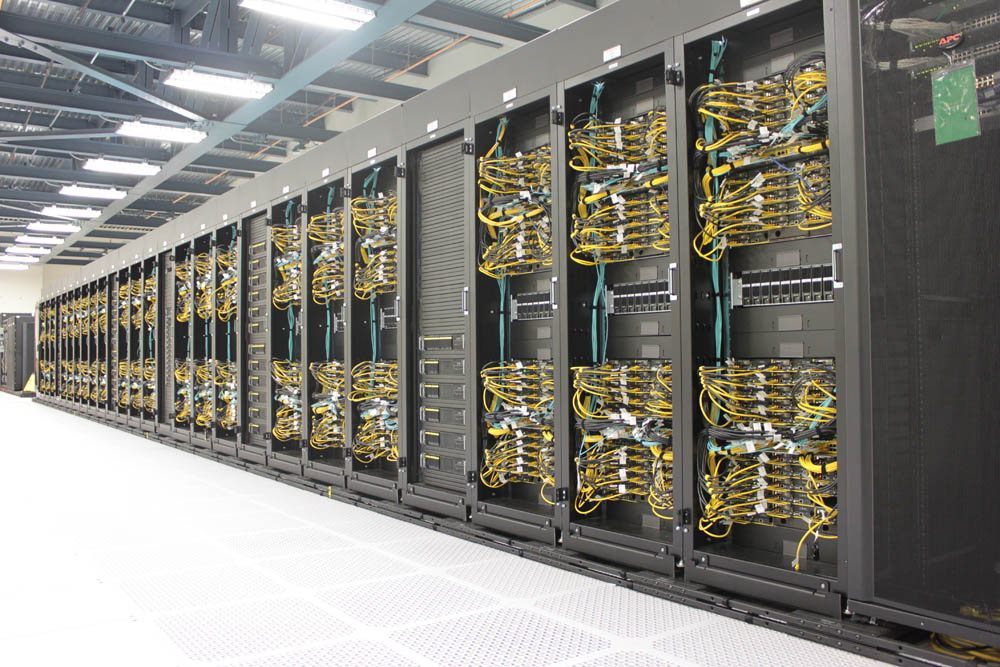
\includegraphics[trim={1cm 5cm 6cm 3cm}, clip, width=\textwidth]{figures/quartz.jpg}
  \caption{Quartz supercomputer at Lawrence Livermore National Laboratory}
  \label{fig:quartz}
\end{figure}

The training data was scaled by calculating the column-wise mean and standard deviation of each discrete variable, subtracting each mean from its corresponding column, and then dividing each column by its corresponding standard deviation.
These last two steps were repeated for the test data using the means and standard deviations from the training data.
The training and test data were then one-hot-encoded using the \textit{dummyVars} function in the \textit{caret} \cite{caret} software package, which converts categorical variables into multi-column dummy variables, where membership within each sub-category is 0 or 1.
The purpose of scaling and one-hot-encoding data was to improve the initial parameter ($\theta$) updates of the neural network \cite{chollet}, and minimize bias towards individual training parameters (Table \ref{table:output2}).

\section{Training Neural Networks}

Each neural network was initially trained for 1,500 epochs using a "mini-batch" training approach \cite{goodfellow}, which consists of splitting the training data into smaller batches of 8,192, computing gradients using \gls{mse} (\ref{eq:mse1}), and updating parameters ($\theta$) after each batch.
Then, each neural network was trained for an additional 150 epochs, and the model was saved as a separate HDF5 file after each epoch.
Lastly, each neural network was evaluated by comparing the sum of mean absolute errors (\ref{eq:mae}) on training and cross-validation data for the last 150 epochs (Figures \ref{fig:train1} and \ref{fig:train2}).
The neural network with the lowest sum of mean absolute errors was selected as the baseline for the neural network metamodel.
To correct for possible bias towards cross-validation data (i.e., the smaller dataset), the weighted averages were also compared (Figures \ref{fig:train-wt1} and \ref{fig:train-wt2}).
Although the sums and weighted averages differ slightly, the selected neural network has the lowest sum and weighted average of mean absolute errors on training and cross-validation data, so there is no change in outcome (Figures \ref{fig:train1}-\ref{fig:train-wt2}).
%
\begin{equation}
  \label{eq:mae}
  \mbox{mean absolute error (MAE)} = \frac{1}{n} \sum_{i = 1}^{n} | x_{observed_{i}} - x_{predicted_{i}} |
\end{equation}

\begin{figure}
  \centering
  \includegraphics[width=\textwidth]{figures/train1.png}
  \caption{Sum of mean absolute errors on training and cross-validation data}
  \label{fig:train1}
  \vspace{+1.1cm}
  \includegraphics[width=\textwidth]{figures/train2.png}
  \caption{Sum of mean absolute errors on training and cross-validation data}
  \label{fig:train2}
\end{figure}

\begin{figure}
  \centering
  \includegraphics[width=\textwidth]{figures/train-wt1.png}
  \caption{Weighted average of mean absolute errors on training and cross-validation data}
  \label{fig:train-wt1}
  \vspace{+1.1cm}
  \includegraphics[width=\textwidth]{figures/train-wt2.png}
  \caption{Weighted average of mean absolute errors on training and cross-validation data}
  \label{fig:train-wt2}
\end{figure}

\subsection{Applying a Sum of Squared Errors Loss Function}

The \gls{mse} loss function (\ref{eq:mse1}) was initially used to train each neural network.
The reason it was used is because nearly all journal articles, preprints
After reading more about loss functions in \textit{The Theory of Point Estimation} \cite{lehmann} and other books \cite{bertsekas,devore,kuhn}, and then failing to find any relevant journal articles or preprints on why MSE is  
Later on, the sum of squared errors loss function (\ref{eq:sse}) was tested, and it was found to outperform the more commonly used \gls{mse} loss function \cite{chollet,goodfellow}.
This section discusses why the sum of squared errors loss function (\ref{eq:sse}) is better, and provides empirical evidence and code to support this claim.
%
\begin{equation}
  \label{eq:sse}
  \mbox{sum of squared errors (SSE)} = \sum_{i = 1}^{n} (x_{observed_{i}} - x_{predicted_{i}})^{2}
\end{equation}

\noindent When a neural network is trained in batches, the number of samples in the last batch is calculated using \textit{n} mod \textit{b}, where \textit{n} is the number of training samples and \textit{b} is batch size.
Typically, this calculation results in a smaller last batch, except in cases where the number of training samples is evenly divisible by batch size.
A smaller last batch isn't a problem by itself, but when the \gls{mse} loss function (\ref{eq:mse1}) is used, the computed gradients are divided by the number of samples in each batch.
This causes the samples in the last batch to be weighted more heavily than all other samples, which causes parameter ($\theta$) updates to become more sensitive to the computed gradients of the last batch.

The effect the last batch has on training stability and overall performance is highly dependent on the optimization algorithm that is used.
A portion of the Adamax optimization algorithm (Algorithm \ref{alg:adamax}) is reproduced in Algorithm \ref{alg:while}, as it is implemented in the neural network metamodel (\ref{sec:nn}, \ref{sec:model}).

\vspace{+0.6cm}
\begin{algorithm}[H]
  \centering
  \caption{Adamax optimization algorithm \textbf{while} loop \cite{kingma}}
  \label{alg:while}
  \begin{algorithmic}
    \STATE \textbf{while} $\theta_{i}$ not converged \textbf{do}
    \STATE \hspace{\algorithmicindent} $i \leftarrow i + 1$
    \STATE \hspace{\algorithmicindent} $g_{i} \leftarrow \bigtriangledown_{\theta} f_{i} (\theta_{i - 1})$ (get gradients from loss function at time step $i$)
    \STATE \hspace{\algorithmicindent} $m_{i} \leftarrow 0.9 \cdot m_{i - 1} + (1 - 0.9) \cdot g_{i}$ (update biased first moment estimate)
    \STATE \hspace{\algorithmicindent} $u_{i} \leftarrow max(0.999 \cdot u_{t - 1}, |g_{i}|)$ (update exponentially weighted infinity norm)
    \STATE \hspace{\algorithmicindent} $\theta_{i} \leftarrow \theta_{t - 1} - (\alpha / (1 - 0.9^{i})) \cdot m_{i} / u_{i}$ (update parameters)
    \STATE \textbf{return} $\theta_{i}$
  \end{algorithmic}
\end{algorithm}

$\beta_{1}$ and $\beta_{2}$ are set to their default values of 0.9 and 0.999, respectively \cite{kingma}.
Under certain circumstances, it might make sense to subsitute each loss function into Algorithm \ref{alg:while} and apply the backpropagation algorithm \cite{goodfellow}.
However, since MSE and SSE are nearly the same, it is much easier to just examine the effect that the leading $\frac{1}{n}$ term (\ref{eq:mse1}) has on the parameter ($\theta$) updates.
The following code was written to perform pseudo parameter ($\theta$) updates under a relatively simple set of assumptions.

% -----------------------
% -----------------------
% -----------------------

The selected neural network was tested using several different optimization algorithms (Figure \ref{fig:opt}) that are available in \textit{TensorFlow} \cite{tensorflow} and other deep learning software packages.
Adamax \cite{kingma} outperformed all other optimization algorithms, as indicated by having the lowest sum of mean absolute errors on training and cross-validation data (Figure \ref{fig:opt}).
The Adamax optimization algorithm was also tested by varying the learning rate ($\alpha$), which is a scaling factor that controls how much the parameters ($\theta$) are updated during training (Figure \ref{fig:lr}).
The default Adamax learning rate is set to 0.002 \cite{tensorflow,chollet,kingma}.
%
\begin{figure}
  \centering
  \includegraphics[width=\textwidth]{figures/opt.png}
  \caption{Training the selected neural network using different optimization algorithms}
  \label{fig:opt}
\end{figure}

\begin{figure}
  \centering
  \includegraphics[width=\textwidth]{figures/lr.png}
  \caption{Training the selected neural network using different learning rates}
  \label{fig:lr}
\end{figure}

When the Adamax learning rate is set to 0.00075, the training error lowers to 1.9e-04, and the cross-validation error remains at 3.4e-04 (Figure \ref{fig:lr}).
As a result, the learning rate was set to 0.00075 to allow for more gradual parameter ($\theta$) updates.
20 neural networks were trained using this learning rate, and the results are plotted and shown in Figures \ref{fig:model}, \ref{fig:remodel}, and \ref{fig:model1}-\ref{fig:model20}.
%
\begin{figure}
  \centering
  \includegraphics[width=\textwidth]{figures/model.png}
  \caption{Training the selected neural network for 1,500 epochs}
  \label{fig:model}
  \vspace{+1.1cm}
  \includegraphics[width=\textwidth]{figures/remodel.png}
  \caption{Training the selected neural network for an additional 150 epochs}
  \label{fig:remodel}
\end{figure}

\section{Model Averaging}

The purpose of using more than one neural network is to reduce generalization error, which is the expected error on new input [41].
This was done by training 50 neural networks separately and then averaging the results of predicted keff values for the test data, which consists of 26,593 output files the neural networks have never seen.
The idea behind this technique, known as model averaging, is that each neural network in the ensemble metamodel will not make the same errors on test data [41].
The expected squared error of the ensemble metamodel, taken from Goodfellow, et al., [41] is shown in Eq. 10 for a set of n regression models with errors % (ϵi) that are drawn from a zero-mean multivariate distribution with variances E[ϵ_i ]=v and covariances E[〖ϵ_i ϵ〗_j ]=c.

If the errors are perfectly correlated, then c = v, and the expected squared error of the ensemble metamodel reduces to v [41].
Conversely, if the errors are perfectly uncorrelated, then c = 0, and the expected squared error reduces to v/n [41].
The ensemble metamodel test errors are plotted and shown in Fig. 14.
